\documentclass[a4paper,11pt]{article}
\usepackage[margin=0.6in]{geometry}
\usepackage{array}
\usepackage{tabularx}
\usepackage{booktabs}
\usepackage{xcolor}
\usepackage{tikz}
\usepackage{fancyhdr}
\usepackage{graphicx}
\usepackage{amsmath}
\usepackage{colortbl}
\usepackage{multirow}
\usepackage{lipsum}

% Define colors
\definecolor{saffron}{RGB}{255,153,51}
\definecolor{darkgreen}{RGB}{19,136,8}
\definecolor{navy}{RGB}{0,0,139}
\definecolor{lightgray}{RGB}{245,245,245}
\definecolor{headerbg}{RGB}{255,248,220}

% Custom commands
\newcommand{\header}[1]{\textbf{\color{navy}#1}}
\newcommand{\subheader}[1]{\textbf{\color{darkgreen}#1}}

\pagestyle{empty}

\begin{document}

% Header with decorative border
\begin{tikzpicture}[overlay, remember picture]
\draw[saffron, line width=3pt] 
  (current page.north west) ++(0.5cm,-0.5cm) -- 
  (current page.north east) ++(-0.5cm,-0.5cm) -- 
  (current page.south east) ++(-0.5cm,0.5cm) -- 
  (current page.south west) ++(0.5cm,0.5cm) -- cycle;
\end{tikzpicture}

% Institution Header
\begin{center}
\colorbox{headerbg}{\parbox{\textwidth}{
\vspace{0.3cm}
\begin{center}
% Logo placeholders
\begin{minipage}{0.15\textwidth}
\centering
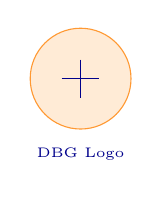
\begin{tikzpicture}[scale=0.8]
\draw[saffron, fill=saffron!20] (0,0) circle (0.8cm);
\draw[navy] (0,0.3) -- (0,-0.3);
\draw[navy] (-0.3,0) -- (0.3,0);
\node[navy] at (0,-1.2) {\tiny DBG Logo};
\end{tikzpicture}
\end{minipage}
\hfill
\begin{minipage}{0.7\textwidth}
\centering
{\Huge\textbf{\color{navy}DIVYA BIHAR GLOBAL GURUKULAM}}\\
{\Large\textbf{\color{darkgreen}(DBG Gurukulam)}}\\
\vspace{0.1cm}
{\large Raghopur, Supaul, Bihar – 852111}\\
{\normalsize Managed by: \textbf{Divya Bihar Mission}}\\
{\small\textit{\color{saffron}Education with Yogic Values}}
\end{minipage}
\hfill
\begin{minipage}{0.15\textwidth}
\centering
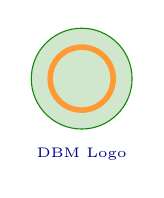
\begin{tikzpicture}[scale=0.8]
\draw[darkgreen, fill=darkgreen!20] (0,0) circle (0.8cm);
\draw[saffron, line width=2pt] (0,0) circle (0.5cm);
\node[navy] at (0,-1.2) {\tiny DBM Logo};
\end{tikzpicture}
\end{minipage}
\end{center}
\vspace{0.3cm}
}}
\end{center}

\vspace{0.3cm}

% Assessment Title
\begin{center}
\colorbox{saffron!20}{\parbox{0.8\textwidth}{
\centering
\vspace{0.2cm}
{\Large\textbf{\color{navy}JIGYASA ANVESHAN III – JULY 2025}}\\
{\large\textbf{\color{darkgreen}Monthly Assessment Report}}
\vspace{0.2cm}
}}
\end{center}

\vspace{0.3cm}

% Student Information
\begin{center}
\begin{tabularx}{\textwidth}{|X|X|X|X|}
\hline
\rowcolor{lightgray}
\header{Student Name:} Shivansh Kumar & \header{Class:} 4th & \header{Roll No:} 12 & \header{Month:} July 2025 \\
\hline
\multicolumn{2}{|c|}{\header{Father's Name:} Ramesh Kumar} & \multicolumn{2}{c|}{\header{Mother's Name:} Sunita Devi} \\
\hline
\end{tabularx}
\end{center}

\vspace{0.3cm}

% Academic Subjects
\begin{center}
\subheader{ACADEMIC SUBJECTS}
\end{center}

\begin{center}
\begin{tabularx}{\textwidth}{|X|c|c|c|c|}
\hline
\rowcolor{navy!20}
\textbf{\color{white}Subject} & \textbf{\color{white}Raw Marks} & \textbf{\color{white}Total} & \textbf{\color{white}Scaled Marks} & \textbf{\color{white}Out of} \\
\hline
Hindi & 42 & 50 & 8.4 & 10 \\
\hline
English & 38 & 50 & 7.6 & 10 \\
\hline
Science & 45 & 50 & 9.0 & 10 \\
\hline
Social Science & 40 & 50 & 8.0 & 10 \\
\hline
Mathematics & 48 & 50 & 9.6 & 10 \\
\hline
Reasoning & 35 & 50 & 7.0 & 10 \\
\hline
\rowcolor{saffron!20}
\textbf{Academic Subtotal} & \textbf{248} & \textbf{300} & \textbf{49.6} & \textbf{60} \\
\hline
\end{tabularx}
\end{center}

\vspace{0.3cm}

% Co-Curricular Activities
\begin{center}
\subheader{CO-CURRICULAR \& EXTRA-CURRICULAR ACTIVITIES}
\end{center}

\begin{center}
\begin{tabularx}{\textwidth}{|X|c|c||X|c|c|}
\hline
\rowcolor{darkgreen!20}
\textbf{\color{white}Activity} & \textbf{\color{white}Marks} & \textbf{\color{white}Out of} & \textbf{\color{white}Activity} & \textbf{\color{white}Marks} & \textbf{\color{white}Out of} \\
\hline
Discipline & 4 & 5 & Project Work & 3 & 5 \\
\hline
Attendance & 5 & 5 & Yoga & 5 & 5 \\
\hline
Class Participation & 4 & 5 & Arts / Painting & 4 & 5 \\
\hline
Oral Performance & 4 & 5 & Fair Copy & 5 & 5 \\
\hline
\multicolumn{6}{|c|}{\cellcolor{saffron!20}\textbf{Co-Curricular Subtotal: 34 / 40}} \\
\hline
\end{tabularx}
\end{center}

\vspace{0.3cm}

% Performance Summary
\begin{center}
\colorbox{navy!10}{\parbox{0.9\textwidth}{
\vspace{0.2cm}
\begin{center}
\subheader{PERFORMANCE SUMMARY}
\end{center}
\begin{center}
\begin{tabularx}{0.85\textwidth}{|X|X|X|X|}
\hline
\rowcolor{saffron!30}
\textbf{Total Marks} & \textbf{Maximum Marks} & \textbf{Percentage} & \textbf{Grade} \\
\hline
83.6 & 100 & 83.6\% & \textbf{Commendable} \\
\hline
\end{tabularx}
\end{center}
\vspace{0.2cm}
}}
\end{center}

\vspace{0.3cm}

% Remarks and Signature Section
\begin{center}
\begin{tabularx}{\textwidth}{|X|}
\hline
\rowcolor{lightgray}
\textbf{Class Teacher's Remarks:} \\
\hline
\rule{0pt}{2.5cm} \\
\hline
\end{tabularx}
\end{center}

\vspace{0.3cm}

% Signature Section
\begin{center}
\begin{tabularx}{\textwidth}{|X|X|X|}
\hline
\rowcolor{lightgray}
\textbf{Class Teacher} & \textbf{Date of Issue} & \textbf{Principal} \\
\hline
\rule{0pt}{2cm} & \rule{0pt}{2cm} & \rule{0pt}{2cm} \\
\hline
\end{tabularx}
\end{center}

\vspace{0.2cm}

% Footer
\begin{center}

\begin{tikzpicture}
\draw[saffron, line width=1pt] (0,0) -- (12,0);
\end{tikzpicture}
\end{center}

\end{document}